%%
%% Kapitel
%%
\chapter{Sprachmodelle}
Bis zur Einf\"uhrung von Sprachmodellen gab es f\"ur NLP in Machine Learning ein gro{\ss}es Problem: Textdaten, wie auch Sprache, sind inherent sequentiell. Im Gegensatz zu Bildern, bei denen alle Daten auf einmal verarbeitet werden k\"onnen, konnte die Textverarbeitung die Beschleunigung durch den Einsatz von GPUs nicht nutzen, da viele Aufgaben nicht parallelisiert werden konnten \cite{attention}.\\ Weiterhin gab es keine M\"oglichkeit, ein schon vortrainiertes Modell f\"ur andere Aufgaben weiter zu verwenden, da das Training f\"ur die verschiedenen Aufgaben und auch Dom\"anen sehr spezifisch angegangen werden muss. Diese Faktoren f\"uhrten zu einem deutlichen Mehraufwand von NLP z.B. gegen\"uber Bildverarbeitung.\\
Das Ziel von Sprachmodellen ist es, parallele Verarbeitung der Daten m\"oglich zu machen sowie, im Gegensatz zu vortrainierten \textbf{Wortvektor Embeddings} wie \textbf{GLoVe} den Kontext der einzelnen W\"orter im Satz zu wahren. In den Embeddings wird jedem Wort ein Vektor zugewiesen, sodass \"ahnliche W\"orter nah beieinander liegen und die Beziehung zwischen W\"ortern erhalten bleibt. Dadurch k\"onnen interessante Rechnungen aufgestellt werden:
\begin{verbatim} 
London - England + Spanien = Madrid
\end{verbatim} 
Mit ganzen Textsequenzen k\"onnen aber auch diese Vektor Embeddings aufgrund der fehlenden Kontextinformationen nur bedingt gut umgehen.
%Transfer Learning
%Sprachgmodelle geben word predictions aus

\section{Problemstellung}
Wie schon erw\"ahnt muss Sprache sequentiell versarbeitet werden. Dazu werden meist \textbf{Gated RNNs} und \textbf{Long Short Term Memory (LSTM)} - Netzwerke verwendet \cite{attention}. Durch einige Techniken kann man mit diesen Netzen auch gute Laufzeiten erreichen, aber es besteht ein weiteres Problem: Der Kontext der W\"orter geht schnell verloren, da diese Netze einem Wort meist auch nur eine Bedeutung zuordnen k\"onnen.Der Umstand, dass diese Netze f\"ur jede Anwendung spezifisch trainiert werden m\"ussen, macht ihren Einsatz sehr umst\"andlich.\\
Ein ebenfalls sehr gro{\ss}es Problem in NLP ist die Tatsache, dass \textbf{\"Uberwachtes Lernen} mit erheblichem manuellen Aufwand - dem Annotieren und Labeln der Daten - verbunden ist. Es gibt zwar sehr gro{\ss}e Mengen an Daten, die durch das Internet verf\"ugbar sind (z.B. alle \textit{Wikipedia-Artikel}, diese eignen sich aber nur f\"ur un\"uberwachte Lernmethoden, da sie nicht gelabelt sind. Die Menge an gelabelten Daten hingegen ist verschwinden gering im Vergleich zu allen frei verf\"ugbaren. Dies legt die Entwicklung eines Systems nahe, das mit \textbf{teil-} oder \textbf{fern\"uberwachtem Lernen} auskommt. Heutige Sprachmodelle versuchen hier anzusetzen, indem sie in einem ersten Schritt un\"uberwacht mit Korpussen unterschiedlicher Gr\"o{\ss}e die Repr\"asentation einer Sprache lernen, um dann im zweiten Schritt an die zu erf\"ullende Aufgabe angepasst zu werden. Interessant hierbei sind neueste Entwicklungen \cite{gpt3}, durch die ein Modell sogar mit nur einem Beispiel der zu erf\"ullenden Aufgabe gute Ergebnisse erzielen kann.

\section{Sprachmodelle auf Basis von LSTMs}
\textbf{LSTMs} k\"onnen aufgrund ihrer Architektur gut mit kurzen S\"atzen umgehen, aber je l\"anger die Wortsequenz, desto schlechter kann sie verarbeitet werden: Es gibt dabei Probleme mit \textbf{vanishing} oder \textbf{exploding gradients}, je nach Einstellung der Parameter.\\
Durch die sequentiellen Verarbeitung steigt die Verarbeitungszeit mit der Textl\"ange an, wodurch \textbf{LSTMs} generell langsamer sind als \textbf{RNNs}, da die Neuronen komplexer sind.\\
Trotz dieser Nachteile k\"onnen mit dieser Architektur f\"ur einige Anwendungen geeignete Sprachmodelle erstellt werden.

\subsection{ELMo}
Prinzipiell ist \textbf{ELMo} eher zu Wortvektoren zu z\"ahlen als zu Sprachmodellen. Die von \textbf{ELMo} erlernten Wort-Embeddings k\"onnen in den eigenen, f\"ur Aufgaben spezifisch entwickelten Netzen eingebunden werden, um gegen\"uber sehr festgelegter Vektoren wir \textbf{GloVe} Ergenisse zu erzielen, die zum Zeitpunkt der Entwicklung dieses Modells zu den besten geh\"orten. Sie wurden abgel\"ost durch die Einf\"uhrung der flexibleren Modelle wie \textbf{BERT}, die schnell bessere Ergebnisse erreichen konnten.

\subsection{ULMFit}

\section{Sprachmodelle auf Basis von Transformern}
\textbf{Transformer} sind die Basis der heute meistgenutzten Sprachmodelle \cite{bert}\cite{gpt}. Sie wurden 2017 entwickelt, um das Problem der sequentiellen Verarbeitung zu l\"osen: Als Eingabe kann ein \textbf{Transformer} eine ganze Textsequenz verarbeiten. Die wichtigste Komponente in diesem System ist \textbf{Attention}: Dadurch kann einem Wort sein Kontext innerhalb der betrachteten Sequenz zugeordnet werden.\\
\begin{figure}[!ht]
\centering
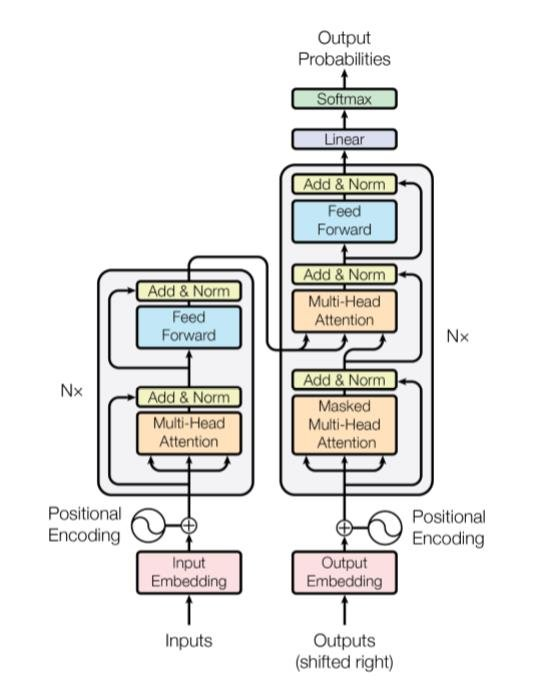
\includegraphics{pics/attention.jpg}
\caption{Aufbau eines Transformers \cite{attention}}
\label{fig:attention}
\end{figure}

\subsection*{Encoder}
Wie in Abbildung \ref{fig:attention} zu sehen, wird die Eingabe zun\"achst in Wortvektoren f\"ur jedes Eingabewort umgewandelt, die sich aus der Addition des Vektors im \textbf{Embedding Space} mit einem \textbf{Positionsvektor (Positional Encoding)}, der die Position des Wortes im Satz enth\"alt, ergibt. Der Positionsvektor wird durch Sinus- und Kosinusfunktionen bestimmt. Dieser Eingabevektor wird an einen \textbf{Encoder} weitergegeben, der eine \textbf{Attention-Matrix} f\"ur die Eingabesequenz erstellt. Sie besteht aus einem Vektor der L\"ange der Textsequenz f\"ur jedes Wort. Diese Matrix enth\"alt Informationen dar\"uber, wie relevant die einzelnen W\"orter der Sequenz f\"ureinander sind: In dem Satz
\begin{verbatim} 
Der braune Hund
\end{verbatim} 
bezieht sich z.B. das Wort "`Der"' sowie das Adjektiv "`braune"' auf das Wort "`Hund"'. In dem Attention-Vektor w\"aren entsprechend die Werte f\"ur "`Hund"' in den Vektoren der beiden anderen W\"orter h\"oher. \textbf{Attention} ist der Schl\"usselpunkt f\"ur die Funktion der Transformer: Dadurch erhalten die Wortvektoren ihre eigentliche Kontextinformation. Um die Werte zu optimieren werden hier die Mittelwerte von acht Vektoren pro Wort ermittelt.\\
Alle bisher errechneten Vektoren werden danach aufaddiert, normalisiert und jeder Vektor wird in ein Feed-Forward-Netz gegeben. Hierbei kann parallelisiert werden, da die einzelnen Vektoren voneinander unabh\"angig sind. Die Ausgabe des \textbf{Encoders} sind die mit Kontext und Attention encodierten Wortvektoren.\\

\subsection*{Decoder}
Der \textbf{Decoder} ist \"ahnlich aufgebaut. Er nimmt einen zweiten Input an - der eigentliche Output bei Supervised Learning - der, wie Abbildung \ref{fig:attention} zeigt, zun\"achst auch in einen Eingabevektor mit Positionsinformation und Attention-Matrix umgewandelt wird. Im n\"achsten Schritt werden Input und Output gemeinsam in ein weiteres Netz zur Attention-Bestimmung gegeben, in dem die Attention Matrix der beiden Vektoren zueinander bestimmt wird: Die Frage die hierbei beantwortet wird ist, wie welche W\"orter in den beiden Sequenzen zueinander stehen. Dies ist gut an dem Beispiel der Sprach\"ubersetzung zu sehen, bei der der zu lernende Output der Input in einer anderen Sprache ist.
\begin{verbatim} 
The brown dog
\end{verbatim} 
w\"are entsprechend hier der Output (Decoder Input). Es wird in diesem Schritt analysiert, wie das Wort "`The"' zu "`Der"', sowie "`braune"' zu "`brown"' und "`Hund"' zu "`dog"' steht.
Diese Vektoren werden wieder aufaddiert, normiert und in ein Feed-Forward-Netz gegeben, um noch einmal addiert und normiert zu werden.\\
Danach wird noch eine lineare und eine Softmax-Schicht angwandt, um am Ende in diesem Beispiel das Wort zu erhalten, dass mit der h\"ochsten Wahrscheinlichkeit als n\"achstes in dem Output-Satz steht. In der Lernphase wird hierzu \textbf{Masking} genutzt, bei dem je ein Wort in dem zu lernenden Ouptut-Satz "`maskiert"', also als leerer Platzhalter markiert wird.



\subsection{GPT}



\subsection{BERT}
%Unterschied zu anderen Modellen
%verschiedene Trainingsmethoden

\section{Weitere Sprachmodelle}

\subsection{XLNet}